% \input{"IAB/latex/TeX-Folienformat.tex"}
\input{"/Users/jonathanlatner/Google Drive/My Drive/IAB/latex/TeX-Folienformat.tex"}

\documentclass[t,8pt,utfx8]{beamer}
\usepackage{booktabs}
\usepackage{setspace}
\usepackage{parskip}
\usepackage{graphicx}
\usepackage{subcaption}
\setbeamertemplate{caption}[numbered]
\newcommand{\sprache}{\englisch}
\renewcommand{\thesubsection}{\alph{subsection})}
\usepackage[cal=pxtx, scr=dutchcal]{mathalpha}


\usepackage{listings} %include R code

\definecolor{codegreen}{rgb}{0,0.6,0}
\definecolor{codegray}{rgb}{0.5,0.5,0.5}
\definecolor{codepurple}{rgb}{0.58,0,0.82}
\definecolor{backcolour}{rgb}{0.95,0.95,0.92}

\lstdefinestyle{mystyle}{
    backgroundcolor=\color{backcolour},   
    commentstyle=\color{codegreen},
    keywordstyle=\color{magenta},
    numberstyle=\tiny\color{codegray},
    stringstyle=\color{codepurple},
    basicstyle=\ttfamily\tiny,
    breakatwhitespace=false,         
    breaklines=true,                 
    captionpos=b,                    
    keepspaces=true,                 
    numbers=left,                    
    numbersep=5pt,                  
    showspaces=false,                
    showstringspaces=false,
    showtabs=false,                 
    columns=fullflexible,
    frame=single,
    tabsize=2
}

\lstset{style=mystyle}


\newcommand{\btVFill}{\vskip0pt plus 1filll}

\title{Generating synthetic data is complicated: Know your data and know your generator}
\subtitle{PSD2024: Privacy in Statistical Databases 2024, \newline 26. September, 2024}

\author{Jonathan Latner, PhD \newline Dr. Marcel Neuenhoeffer \newline Prof. Dr. Jörg Drechsler}

\newcounter{noauthorlines}
\setcounter{noauthorlines}{2} % Wert für 2 Autoren über 2 Zeilen. Ggf. anpassen

% %%%%%%%%%%%%%%
% Ende Anpassung
% %%%%%%%%%%%%%%

% \input{"IAB/latex/TeX-Folienformatierung_CD_2019"}
\input{"/Users/jonathanlatner/Google Drive/My Drive/IAB/latex/TeX-Folienformatierung_CD_2019"}

% Modify the section in toc template to enumerate
\setbeamertemplate{section in toc}{%
    \inserttocsectionnumber.~\inserttocsection\par
}

% use for subsections
% \setbeamertemplate{subsection in toc}{}
\setbeamertemplate{subsection in toc}{%
    \setlength{\parskip}{1mm}
        \hskip2mm -- \hskip1mm\inserttocsubsection\par
}


\usepackage{colortbl}
\definecolor{lightgray}{gray}{0.9}


\begin{document}


\frame[plain]{\titlepage}

\begin{spacing}{1.25}


\section{Introduction}\label{sec:intro}
\begin{frame}[c,plain]
\vskip-4mm
\begin{beamercolorbox}[wd=\boxwidth,ht=22.11mm]{transparent}%
    \vfill%
    \usebeamerfont{title}%
    \leftinsert%
    \MakeUppercase{Section \ref{sec:intro}: Introduction
} % <- Hier die Überschrift eintragen
\end{beamercolorbox}
\vskip-3mm
\pgfuseimage{rahmenlinie}
\end{frame}

\frame{\frametitle{Overview}

\begin{itemize}
    \item Common perception that making synthetic data is easy
    \item We to show that its complicated
    \begin{itemize}
        \item You need to know your data
        \begin{itemize}
            \item Missing values, messy data, etc.
        \end{itemize}
        \item You need to know your synthetic data generator (SDG)
        \begin{itemize}
            \item Compare 3 SDGs: DataSynthesizer, CTGAN, Synthpop
            \item How does it deal with missing values?
            \item How computationally efficient is it (in terms of duration in time)?
        \end{itemize}
    \end{itemize}
    \item Conclusion
    \begin{itemize}
        \item On the one hand, generating synthetic data is easy (even I can do it!)
        \item On the other hand, users need to be aware of challenges
        \item Every SDG has advantages/disadvantages (no one, correct solution)
        \item One should be skeptical about automated processes for generating synthetic data
    \end{itemize}
\end{itemize}
}

\frame{\frametitle{The good news -- making synthetic data is easy}

\begin{itemize}
    \item \url{Gretel.ai}: The synthetic data platform for developers. Generate artificial datasets with the same characteristics as real data, so you can develop and test AI models without compromising privacy.
    \item \url{Mostly.ai}: Synthetic Data. Better than real. Still struggling with real data? Use existing data for synthetic data generation. Synthetic data is more accessible, more flexible, and simply...smarter.
    \item \url{Statice.ai}: Generating synthetic data comes down to learning the joint probability distribution in an original, real dataset to generate a new dataset with the same distribution.  The more complex the real dataset, the more difficult it is to map dependencies correctly. Deep learning models such as generative adversarial networks (GAN) and variational autoencoders (VAE) are well suited for synthetic data generation.
    \item \url{hazy.com}: Synthetic data does not contain any real data points so can be shared freely. Say goodbye to lengthy governance processes associated with real data.  Specifically, Hazy data is designed to preserve all the patterns, statistical properties and correlations in the source data, so that it can be used as a drop-in replacement for it.
    \item DataSynthesizer (Ping et al., 2017): The distinguishing feature of DataSynthesizer is its usability — the data owner does not have to specify any parameters to start generating and sharing data safely and effectively.
\end{itemize}
}

\frame{\frametitle{The bad news -- making synthetic data is hard}

\begin{itemize}
    \item According to the Alan Turing Institute (Jordan et al., 2022)
    \item Synthetic data is not a replacement for real data.  It is a distorted version of the real data.
    \item We must ask: 
    \begin{itemize}
        \item Why are we creating synthetic data?  
        \item How different should it be?  
        \item How do we measure the difference?  
        \item How does the synthesizer work? 
    \end{itemize}
    \item Answering these questions will help us make decisions about which synthesizer is the right choice
    \begin{itemize}
        \item Hyperparameters: from complete black box to complete user choice
        \item Variables: not just with categorical, dichotomous, and continuous variables, but with messy values 
        \item Computationally efficiency (i.e. duration in time): is important and often ignored.  The algorithm should scale well with the dimension of the data space in a relational way, not exponential way.
    \end{itemize}
\end{itemize}
}



\frame{\frametitle{Our goal is to illustrate the challenges}
\begin{itemize}
    \item Know your data (1 dataset)
    \begin{itemize}
        \item Social Diagnosis 2011 (SD2011) - Cleaning/pre-processing (most evaluations use clean data)
    \end{itemize}
    \item Know your generator
    \begin{itemize}
        \item Compare 3 synthetic data generators (SDGs): DataSynthesizer, CTGAN, Synthpop
    \end{itemize}
    \item 3 utility measures
    \begin{itemize}
        \item Compare univariate frequency
        \item Propensity score mean-squared error (pMSE) - Append the original and synthetic datasets. Create an indicator variable for original/synthetic datasets.  The probability of being in the synthetic dataset is computed for each record in the combined dataset ($n$); this is the propensity score ($p$).  Lower scores are better.  ($pMSE = \frac{1}{N}\sum_{i=1}^{N}[\hat{p}_i - c]^2$)
        \item Computationally efficient with respect to duration in time
    \end{itemize}
    \item In this talk, we are focusing on utility.  Relative to the challenge of achieving privacy, utility challenges receive less attention.
\end{itemize}
}


\section{Know your data (SD2011)}\label{sec:data}
\begin{frame}[c,plain]
\vskip-4mm
\begin{beamercolorbox}[wd=\boxwidth,ht=22.11mm]{transparent}%
    \vfill%
    \usebeamerfont{title}%
    \leftinsert%
    \MakeUppercase{Section \ref{sec:data}: Know your data (SD2011)} % <- Hier die Überschrift eintragen
\end{beamercolorbox}
\vskip-3mm
\pgfuseimage{rahmenlinie}
\end{frame}


\frame{\frametitle{Real data}
\begin{itemize}
    \item Social Diagnosis 2011 (SD2011)
    \item Loads with Synthpop
    \begin{itemize}
        \item \url{http://www.diagnoza.com/index-en.html}
        \item Not entirely clear how original data is created or cleaned to create data in Synthpop
        \begin{itemize}
            \item No 
        \end{itemize}
    \end{itemize}
    \item Like real data, has `quirks' or unusual values/variables
    \begin{itemize}
        \item Includes missings
        \begin{itemize}
            \item Informative (i.e. for never worked abroad, \texttt{wkabdur} is missing)
            \item Non-informative 
        \end{itemize}
        \item Includes `errors'
        \begin{itemize}
            \item \texttt{smoke} - Does smoke is NO, but \texttt{nociga} - 20/22 cigarettes per day 
            \item \texttt{bmi} = 451, but \texttt{height}(cm) = 149 and \texttt{weight}(kg) = NA (999)
        \end{itemize}
        \item Includes generated variables (Can be problematic for SDGs)
        \begin{itemize}
            \item \texttt{bmi,agegr}
        \end{itemize}
    \end{itemize}
\end{itemize}
}


\frame{\frametitle{Data (SD2011)}
\begin{table}[ht]
    \vskip -3mm
    \caption{Spikey values}
    \centering
    \vskip -7mm
    \rowcolors{1}{white}{lightgray}
    \resizebox{\textwidth}{!}{% latex table generated in R 4.4.0 by xtable 1.8-4 package
% Thu Sep 26 09:11:53 2024
\begin{tabular}{rlllllllll}
  \toprule
Number & Variable & Description & Type & Observations & Unique.Values & Missings & Negative.values & Generated & Messy \\ 
  \midrule
  1 & sex & Sex & factor & 5000 & 2 & 0 & 0 &  &  \\ 
    2 & age & Age of person, 2011 & numeric & 5000 & 79 & 0 & 0 &  &  \\ 
    3 & agegr & Age group, 2011 & factor & 5000 & 7 & 4 & 0 & Yes & Yes \\ 
    4 & placesize & Category of the place of residence & factor & 5000 & 6 & 0 & 0 &  &  \\ 
    5 & region & Region (voivodeship) & factor & 5000 & 16 & 0 & 0 &  &  \\ 
    6 & edu & Highest educational qualification, 2011 & factor & 5000 & 5 & 7 & 0 &  &  \\ 
    7 & eduspec & Discipline of completed qualification & factor & 5000 & 28 & 20 & 0 &  &  \\ 
   &  &  &  & \dots &  &  &  &  &  \\ 
   10 & income & Personal monthly net income & numeric & 5000 & 407 & 683 & 603 &  & Yes \\ 
   11 & marital & Marital status & factor & 5000 & 7 & 9 & 0 &  &  \\ 
   12 & mmarr & Month of marriage & numeric & 5000 & 13 & 1350 & 0 &  &  \\ 
   14 & msepdiv & Month of separation/divorce & numeric & 5000 & 13 & 4300 & 0 &  &  \\ 
   15 & ysepdiv & Year of separation/divorce & numeric & 5000 & 51 & 4275 & 0 &  &  \\ 
   &  &  &  & \dots &  &  &  &  &  \\ 
   22 & nofriend & Number of friends & numeric & 5000 & 44 & 0 & 41 &  & Yes \\ 
   23 & smoke & Smoking cigarettes & factor & 5000 & 3 & 10 & 0 &  &  \\ 
   24 & nociga & Number of cigarettes smoked per day & numeric & 5000 & 30 & 0 & 3737 &  & Yes \\ 
   &  &  &  & \dots &  &  &  &  &  \\ 
   28 & wkabdur & Total time spent on working abroad & numeric & 5000 & 33 & 0 & 4875 &  & Yes \\ 
   &  &  &  & \dots &  &  &  &  &  \\ 
   33 & height & Height of person & numeric & 5000 & 65 & 35 & 0 &  &  \\ 
   34 & weight & Weight of person & numeric & 5000 & 91 & 53 & 0 &  &  \\ 
   35 & bmi & Body mass index (weight - kg/(height - cm$^2$)*10000) & numeric & 5000 & 1396 & 59 & 0 & Yes & Yes \\ 
   \bottomrule
\end{tabular}
}
    \label{table:sd2011_data_structure}
\end{table}
}

\section{Know your generator}\label{sec:sdg}
\subsection{DataSynthesizer}\label{sec:sdg_datasynthesizer}
\begin{frame}[c,plain]
\vskip-4mm
\begin{beamercolorbox}[wd=\boxwidth,ht=22.11mm]{transparent}%
    \vfill%
    \usebeamerfont{title}%
    \leftinsert%
    \MakeUppercase{Section \ref{sec:sdg}\ref{sec:sdg_datasynthesizer}: Know your generator (DataSynthesizer)} % <- Hier die Überschrift eintragen
\end{beamercolorbox}
\vskip-3mm
\pgfuseimage{rahmenlinie}

DataSynthesizer is a Python package that implements the PrivBayes algorithm to address the challenges associated with a differentially private (DP) method for releasing synthetic data outputs from high-dimensional real data inputs. To do this, the package implements a Bayesian network model to estimate the joint distribution of the data.  The Bayesian network only works with discrete variables. One way to discretize continuous variables is by binning them.  This can be a problem.

\begin{itemize}
    \item Hyperparameters
    \begin{itemize}
        \item $\epsilon$ Differential Privacy (DP): we turn it off (default 0.1)
        \item $k$-degree Bayesian network (parents): 2 (default is `greedy')
    \end{itemize}
    \item Utility measure - compare univariate frequency between original and synthetic data
\end{itemize}
\end{frame}



\frame{\frametitle{Preprocess missing values}
\begin{figure}
    \caption{Captures values $<$ 0 as continuous, not missing/categorical}
    \vskip -2mm
    \resizebox{\textwidth}{!}{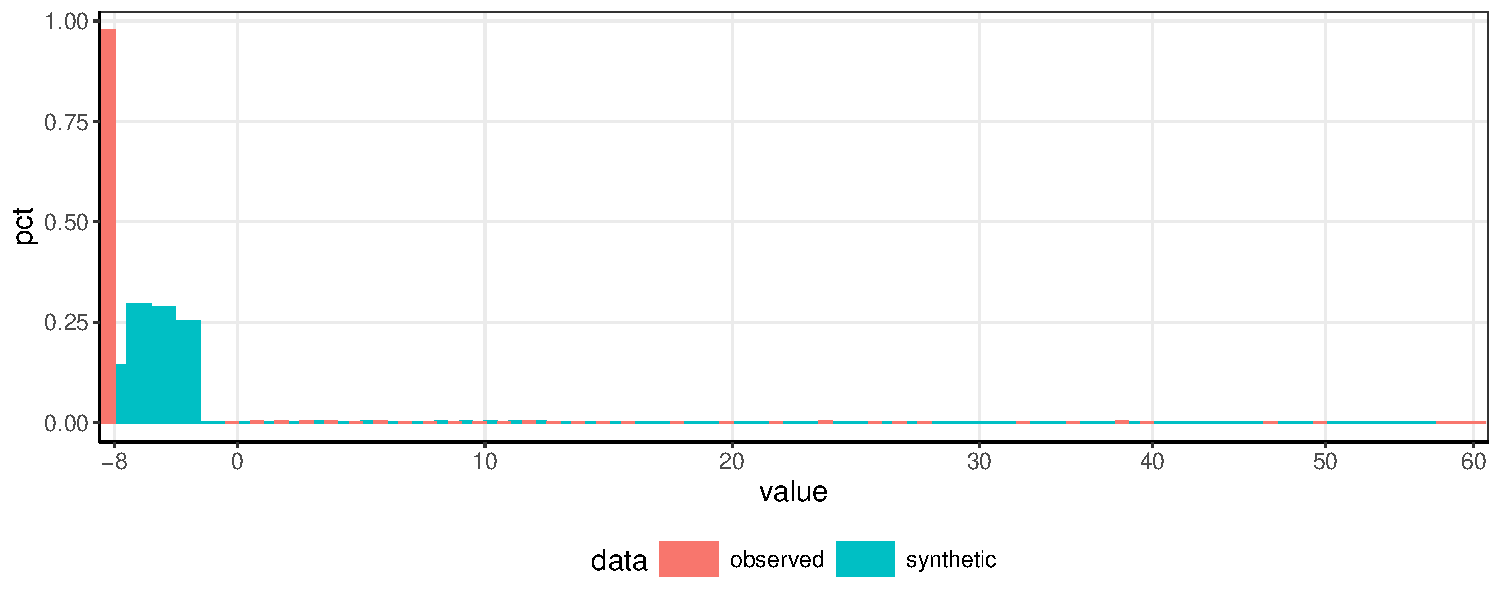
\includegraphics{../../graphs/datasynthesizer_wkabdur.pdf}}
    \label{fig:ds_variable_wkabdur}
\end{figure}
}

\frame{\frametitle{Drop generated variables (1 of 2)}
\begin{figure}
    \caption{Age group: Number of misclassified}
    \vskip -2mm
    \resizebox{\textwidth}{!}{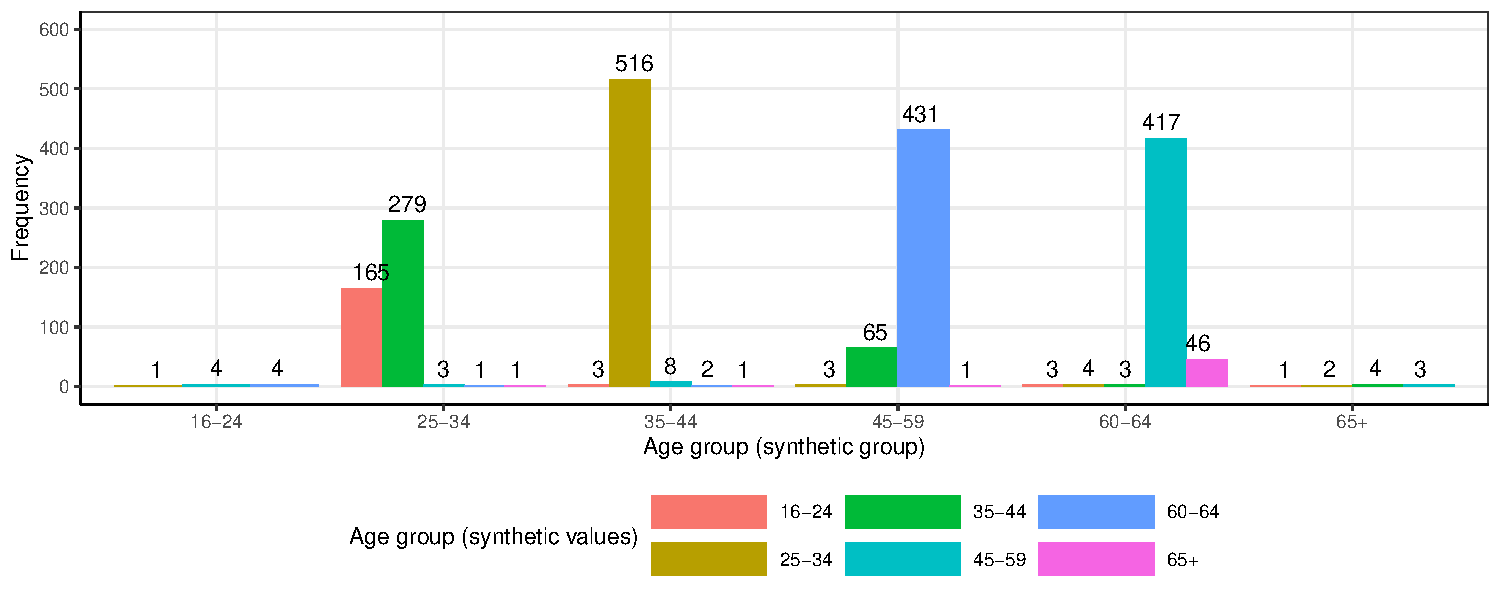
\includegraphics{../../graphs/datasynthesizer_frequency_agegr_errors.pdf}}
    \label{fig:ds_agegr_errors}
\end{figure}
}

\frame{\frametitle{Drop generated variables (2 of 2)}
\begin{figure}
    \caption{BMI: Preprocess extreme values}
    \vskip -2mm
    \resizebox{\textwidth}{!}{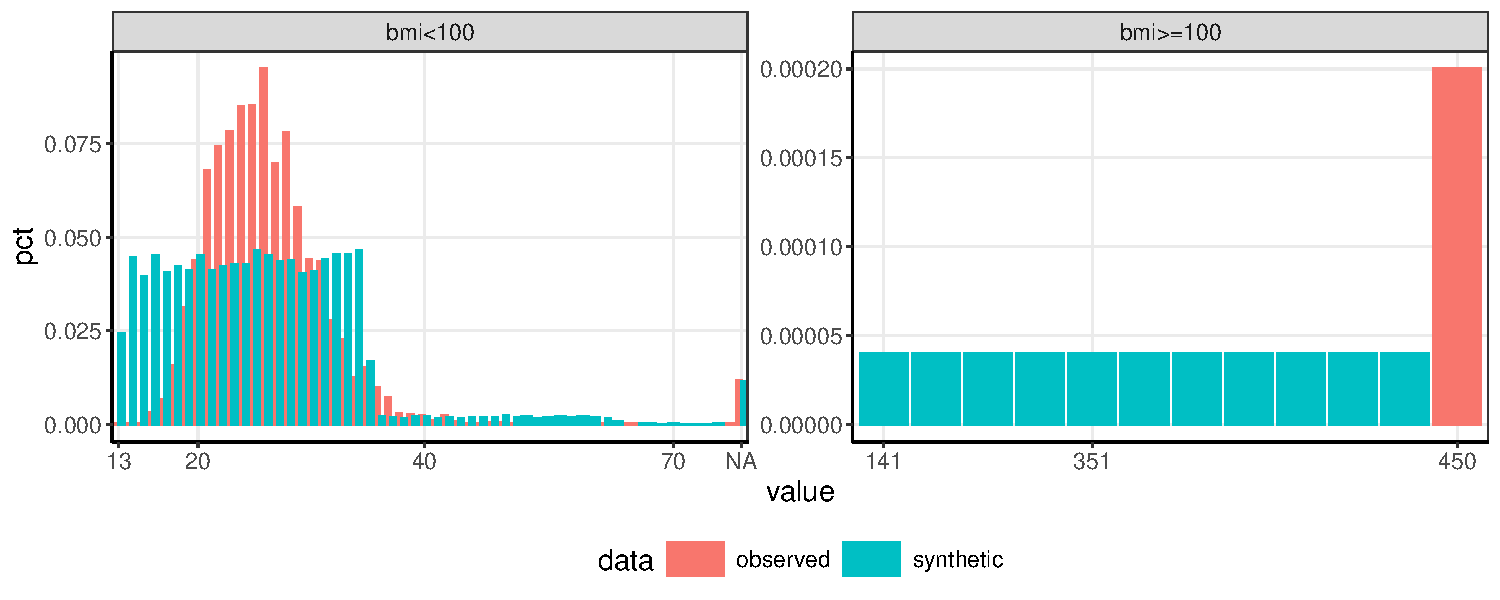
\includegraphics{../../graphs/datasynthesizer_bmi.pdf}}
    \label{fig:ds_bmi}
\end{figure}
}

\frame{\frametitle{Regenerate generated variables from synthetic values}
\begin{figure}
    \caption{Body mass index}
    \vskip -2mm
    \resizebox{\textwidth}{!}{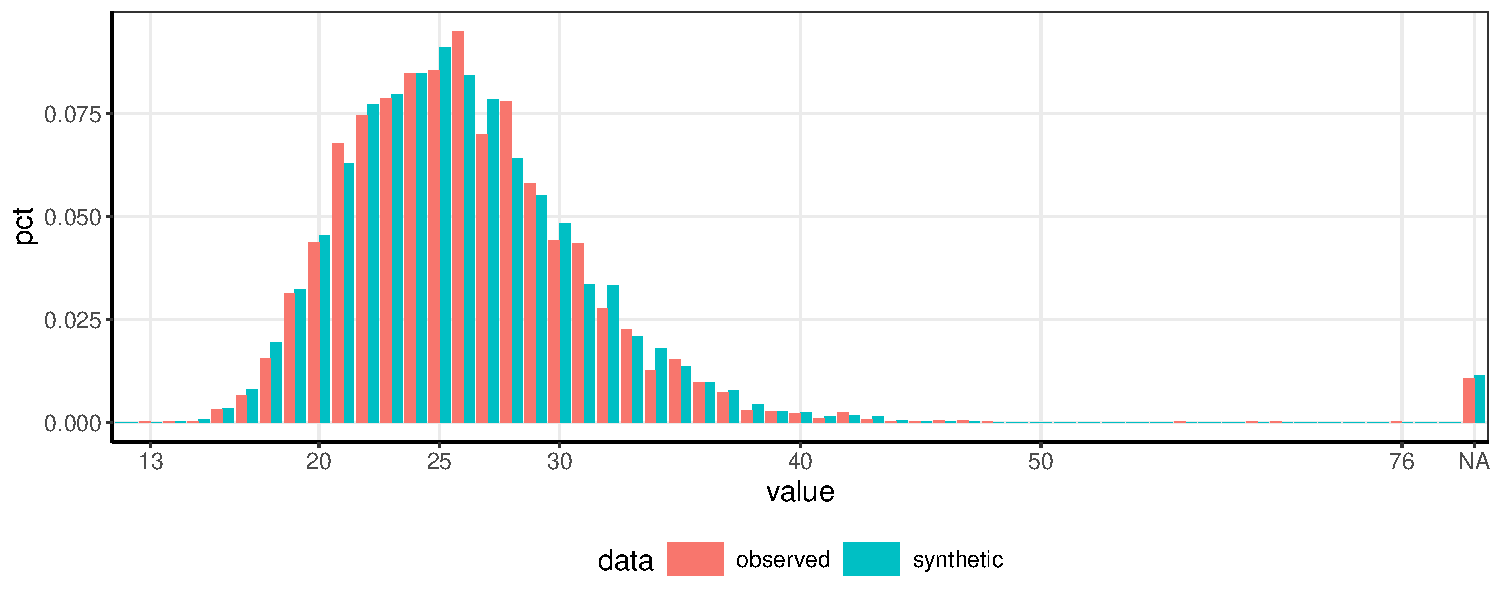
\includegraphics{../../graphs/compare_ds_bmi.pdf}}
    \label{fig:compare_ds_bmi.pdf}
\end{figure}
}


\frame{\frametitle{Can only preprocess so much}
\begin{figure}
    \caption{nofriend: `Spikey' or discontinuous values}
    \vskip -2mm
    \resizebox{\textwidth}{!}{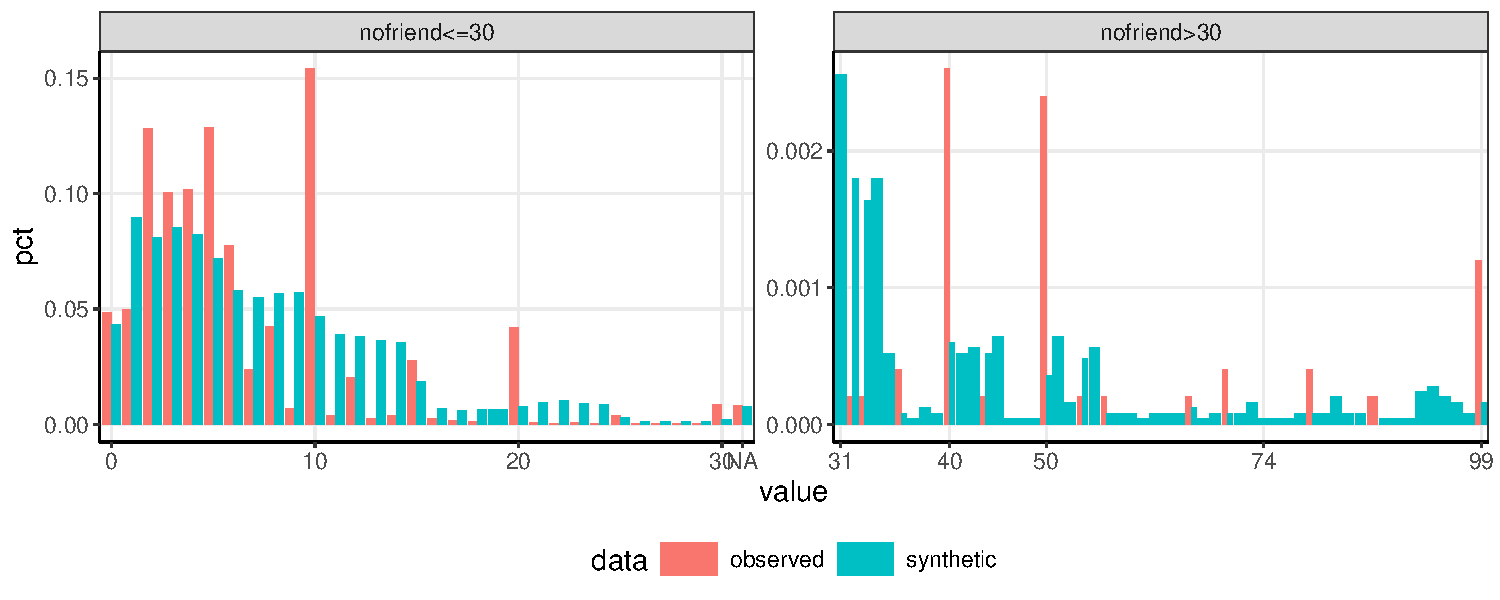
\includegraphics{../../graphs/datasynthesizer_nofriend.pdf}}
    \label{fig:ds_nofriend}
\end{figure}
}


\subsection{CTGAN}\label{sec:sdg_ctgan}
\begin{frame}[c,plain]
\vskip-4mm
\begin{beamercolorbox}[wd=\boxwidth,ht=22.11mm]{transparent}%
    \vfill%
    \usebeamerfont{title}%
    \leftinsert%
    \MakeUppercase{Section \ref{sec:sdg}\ref{sec:sdg_ctgan}: Know your generator (CTGAN)} % <- Hier die Überschrift eintragen
\end{beamercolorbox}
\vskip-3mm
\pgfuseimage{rahmenlinie}

GANs simultaneously train two neural networks: a generator and a discriminator. The goal of the generator is to create synthetic data that becomes increasingly indistinguishable from original data. The goal of the discriminator is to get better at distinguishing between original and synthetic data. This adversarial process goes back and forth until the discriminator cannot distinguish between the original data and the generated data.


\begin{itemize}
    \item Hyperparameters
    \begin{itemize}
        \item Actual steps for observations ($n$) = $f$ (batch * steps per epoch * epochs) 
        \begin{itemize}
            \item batch size = Number of samples to process in each step (default is 500)
            \item epochs = Number of times the GAN gets to see the full dataset (default is 300).
        \end{itemize}
        \item Dimensions
        \begin{itemize}
            \item Discriminator/Generator - defines the architecture of the Discriminator by specifying the number of neurons in each layer. Defaults to (256, 256)
            \item Embeddings - Size of the random sample passed to the Generator. (Default 128)
        \end{itemize}
    \end{itemize}
    \item Utility - pMSE
\end{itemize}

\end{frame}

\frame{\frametitle{Vary batch size, but steps are constant (3000)}
\begin{figure}
    \caption{DataSynthesizer (0.07) and Synthpop (0.02)}
    \vskip -2mm
    \resizebox{\textwidth}{!}{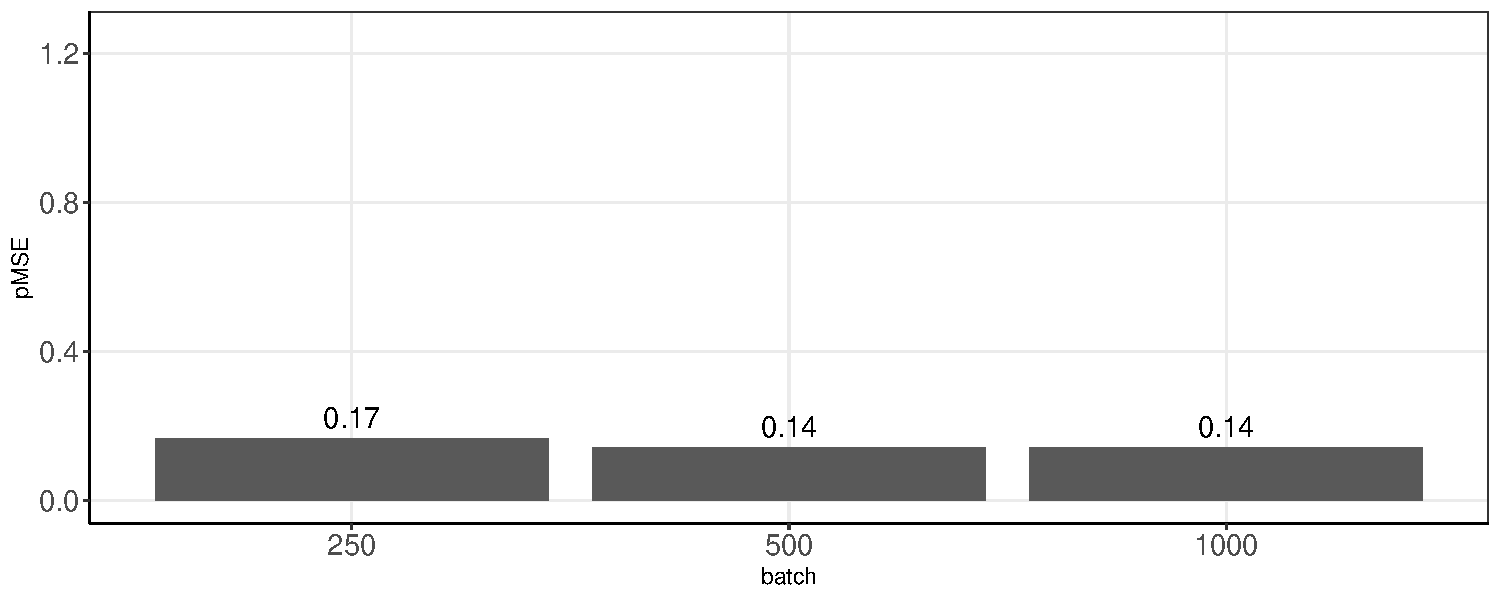
\includegraphics{../../graphs/ctgan_fidelity_optimize_batch_size.pdf}}
    \label{fig:ctgan_fidelity_optimize_batch_size.pdf}
\end{figure}
}


\frame{\frametitle{Vary epochs, but batch size is constant (500)}
\begin{figure}
    \caption{DataSynthesizer (0.07) and Synthpop (0.02)}
    \vskip -2mm
    \resizebox{\textwidth}{!}{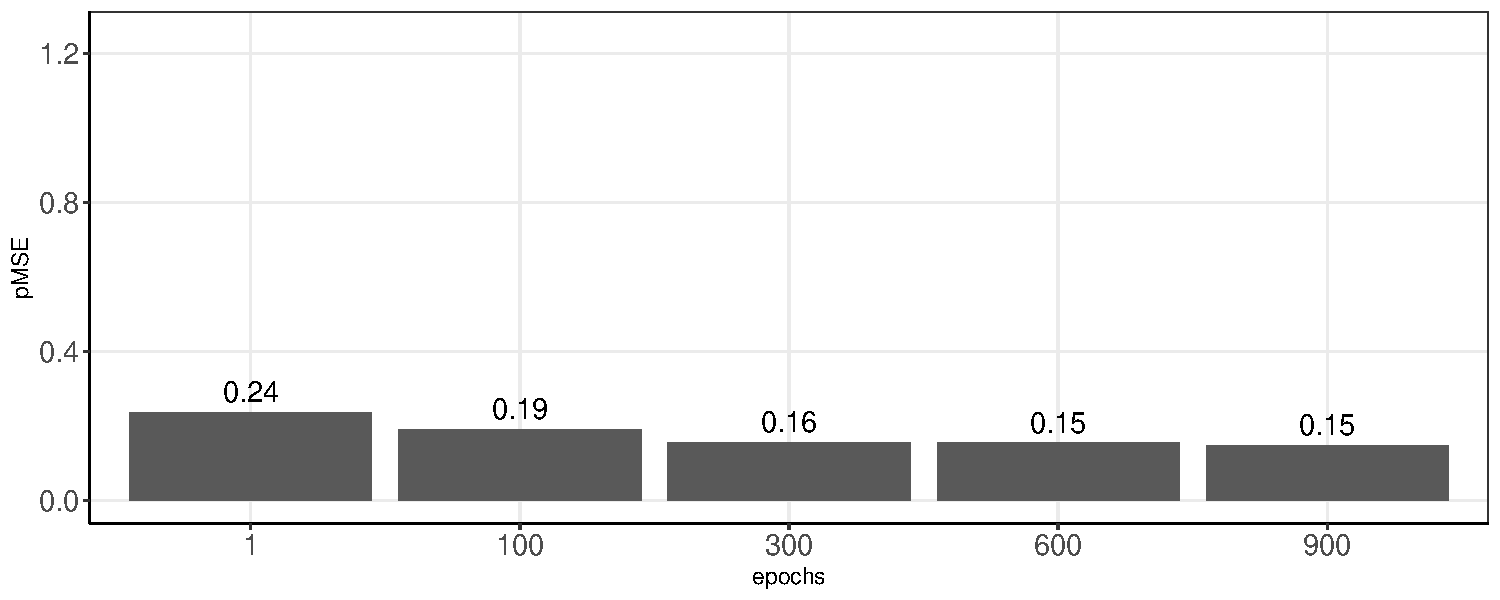
\includegraphics{../../graphs/ctgan_fidelity_optimize_epochs.pdf}}
    \label{fig:ctgan_fidelity_optimize_epochs}
\end{figure}
}

\frame{\frametitle{Optimize dimensions}
\begin{figure}
    \caption{DataSynthesizer (0.07) and Synthpop (0.02)}
    \vskip -2mm
    \resizebox{\textwidth}{!}{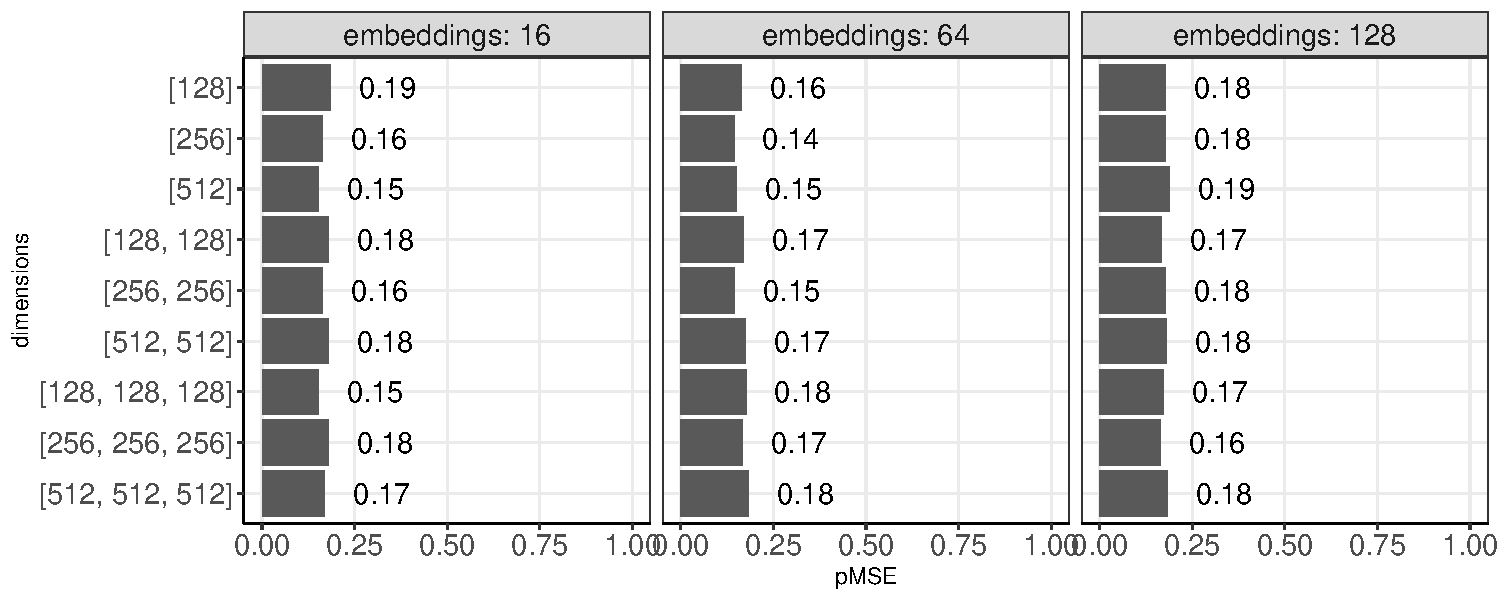
\includegraphics{../../graphs/ctgan_fidelity_optimize_dimensions.pdf}}
    \label{fig:ctgan_fidelity_optimize_dimensions}
\end{figure}
}


\subsection{Synthpop}\label{sec:sdg_synthpop}
\begin{frame}[c,plain]
\vskip-4mm
\begin{beamercolorbox}[wd=\boxwidth,ht=22.11mm]{transparent}%
    \vfill%
    \usebeamerfont{title}%
    \leftinsert%
    \MakeUppercase{Section \ref{sec:sdg}\ref{sec:sdg_synthpop}: Know your generator (Synthpop)} % <- Hier die Überschrift eintragen
\end{beamercolorbox}
\vskip-3mm
\pgfuseimage{rahmenlinie}

Synthpop is an R package that implements parametric and ML based models (classification and regression trees (CART) and random forests) to generate synthetic data. Synthpop follows a sequential process, where the first variable to be synthesized is generated by drawing new values from the marginal distribution of this variable (either by drawing from a parametric distribution or by sampling from the empirical distribution), and the subsequent variables are synthesized one at a time, always conditioning on those variables that have been synthesized in earlier steps

\begin{itemize}
    \item Hyperparameters (default)
    \item Utility measure - Computational efficiency
\end{itemize}

\end{frame}

\frame{\frametitle{Computational efficiency}
\begin{table}[ht]
    \vskip -2mm
    \caption{Synthpop may have lowest pMSE, but is not as efficient with high dimensional data}
    \vskip -5mm
    \rowcolors{1}{white}{lightgray}
    \resizebox{\textwidth}{!}{% latex table generated in R 4.4.0 by xtable 1.8-4 package
% Fri Jul 19 16:14:31 2024
\begin{tabular}{llrrrr}
  \toprule
version & description & ctgan & datasynthesizer & synthpop (csv) & synthpop (package) \\ 
  \midrule
v00 & Raw (SD2011) & 331.01 & 245.37 & 2132.12 & 5474.39 \\ 
  v01 & Without eduspec or wkabdur & 290.30 & 264.43 & 10.99 & 8.45 \\ 
  v02 & Without wkabdur & 337.07 & 351.76 & 13.96 & 11.02 \\ 
  v03 & Without eduspec & 306.46 & 351.24 & 11.39 & 8.92 \\ 
  v04 & Last variables: eduspec-wkabdur & 374.57 & 344.02 & 14.23 & 287.85 \\ 
  v05 & Last variables: wkabdur-eduspec & 419.60 & 339.92 & 14.60 & 3657.55 \\ 
  v06 & as.numeric(wkabdur) and last variable: eduspec & 356.02 & 347.36 & 14.12 & 11.05 \\ 
  v07\_1\_20 & + 1 factor variable (20 values) & 339.05 & 264.96 & 42.23 &  \\ 
  v07\_1\_25 & + 1 factor variable (25 values) & 400.28 & 326.84 & 137.47 &  \\ 
  v07\_1\_30 & + 1 factor variable (30 values) & 339.73 & 269.72 & 363.18 &  \\ 
  v07\_2\_20 & + 2 factor variable (20 values) & 369.74 & 339.45 & 74.96 &  \\ 
  v07\_2\_25 & + 2 factor variable (25 values) & 364.56 & 361.81 & 631.43 &  \\ 
  v07\_2\_30 & + 2 factor variable (30 values) & 373.25 & 346.15 & 1222.54 &  \\ 
  v07\_3\_20 & + 3 factor variable (20 values) & 393.99 & 369.58 & 122.77 &  \\ 
  v07\_3\_25 & + 3 factor variable (25 values) & 401.03 & 383.40 & 881.53 &  \\ 
  v07\_3\_30 & + 3 factor variable (30 values) & 394.44 & 424.64 & 3654.59 &  \\ 
   \bottomrule
\end{tabular}
}
    \label{table:table_sd2011_duration_v2}
\end{table}
}

\section{Conclusion}\label{sec:conclusion}
\begin{frame}[c,plain]
\vskip-4mm
\begin{beamercolorbox}[wd=\boxwidth,ht=22.11mm]{transparent}%
    \vfill%
    \usebeamerfont{title}%
    \leftinsert%
    \MakeUppercase{Section \ref{sec:conclusion}: Conclusion} % <- Hier die Überschrift eintragen
\end{beamercolorbox}
\vskip-3mm
\pgfuseimage{rahmenlinie}

\end{frame}


\frame{\frametitle{Summary}

\begin{itemize}
    \item You need to know your data 
    \begin{itemize}
        \item Missing values, Extreme values, Generated variables, `Spikey' or discontinuous values
    \end{itemize}
    \item You need to know your synthesizer
    \begin{itemize}
        \item CTGAN 
        \begin{itemize}
            \item Pro: high levels of computational efficiency
            \item Con: GAN architecture may not produce synthetic data with high levels of utility, at least in low dimensional data (33 columns, 5000 rows).
        \end{itemize}
        \item DataSynthesizer uses a Bayesian network model.
        \begin{itemize}
             \item Pro: high levels of computational efficiency
             \item Con: algorithm assumes all variables are discrete, which reduces utility of synthetic continuous variables. 
         \end{itemize} 
        \item Synthpop 
        \begin{itemize}
             \item Pro: high levels of utility (pMSE)
             \item Con: CART struggles with computational efficiency on datasets that contain variables with many categories. 
         \end{itemize} 
    \end{itemize}
    \item The people who know the data may not understand the synthesizer and vice versa
\end{itemize}
}


\end{spacing}
\end{document}

